\documentclass[handout]{beamer}
% L'option handout permet de supprimer la barre de navigation

\usepackage[T1]{fontenc}
\usepackage[utf8]{inputenc}
\usepackage[french]{babel}
% Pour utiliser le signe €
\usepackage{eurosym}
% Pour pouvoir insérer des images
\usepackage{graphicx}
\usepackage{wrapfig}
% Gestion des couleurs
\usepackage{color}
\definecolor{QTPurple}{RGB}{61, 68, 160}
% Coloration syntaxique
\usepackage{listings}

% Un joli thème flat
\usetheme{Rochester}

% Personnalisation du thème
\usecolortheme[named=QTPurple]{structure}
\setbeamertemplate{blocks}[shadow=false]

% Affichage du logo Quantic Télécom en bas de chaque slide
\newif\ifplacelogo % create a new conditional
\placelogotrue % set it to true
\logo{\ifplacelogo
\includegraphics[height=10mm]{images/logo.png}\fi}

% ------------------------------------ %
% -- METADONNÉES DU DOCUMENT --------- %
\title[Quantic]{
	Présentation de Quantic Télécom\\
}
\author{
	Antoine Augusti - \underline{antoine@quantic-telecom.net}
}
\date{12 mars 2014}

\titlegraphic{
\includegraphics[height=.3\textheight]{images/logo.png}}

% Début du document
\begin{document}
	
	% Génération de la page de titre
	\begin{frame}[plain]
		\titlepage
	\end{frame}

	% Génération du sommaire
	\begin{frame}[plain]
		\frametitle{Sommaire}
		\tableofcontents
	\end{frame}


	% ///////////////////////////////////////////////////////// %
	% /// Quantic Télécom c'est quoi ? /////////////////////// %
	\section{Quantic Télécom c'est quoi ?}

	\subsection{La création}
		\begin{frame}
		\frametitle{La création}
		\begin{tabular}{l l}
			\begin{minipage}{0.2\textwidth}
				\begin{center}
					
\includegraphics[width=0.9\textwidth]{images/internet.png}
				\end{center}
			\end{minipage}

			\begin{minipage}{0.8\textwidth}
				\begin{itemize}
					\item \textbf{opérateur} et \textbf{FAI associatif} créé en sept. 2011
					\item arrivée à l'INSA de Rouen après le bac
					\begin{itemize}
						\item pas de connexion \textit{Internet}, au mieux du \textit{web}
						\item acquisition d'une nouvelle résidence par l'INSA
					\end{itemize}
					\item une dizaine de geeks motivés et \textit{un peu} fous
					\item déclaration ARCEP dans la foulée
					\item création sans subvention et sans apport financier
				\end{itemize}
			\end{minipage}
			
		\end{tabular}
		\end{frame}

	\subsection{Public couvert aujourd'hui}
		\begin{frame}
		\frametitle{Public couvert aujourd'hui}
		\begin{tabular}{l l}
			\begin{minipage}{0.2\textwidth}
				\begin{center}
					
\includegraphics[width=0.9\textwidth]{images/residence.png}
				\end{center}
			\end{minipage}

			\begin{minipage}{0.8\textwidth}
				\begin{itemize}
					\item couverture des 5 résidences de l'INSA de Rouen
					\item présent dans 2 résidences du CROUS : Malibran et Emma Bovary
					\item 650 adhérents cette année
					\item 7 personnes impliquées dans le projet
					\item présent dans 2 \textit{datacenters} : Cogent (Rouen), TH2 (Paris)
				\end{itemize}
			\end{minipage}
			
		\end{tabular}
		\end{frame}

	% //////////////////////////////////////////// %
	% /// Le réseau actuel /////////////////////// %
	\section{Le réseau actuel}

	\subsection{Comment relier les résidences ?}
		\begin{frame}
		\frametitle{Comment relier les résidences ?}
		\vspace{-5px}
		\begin{center}
			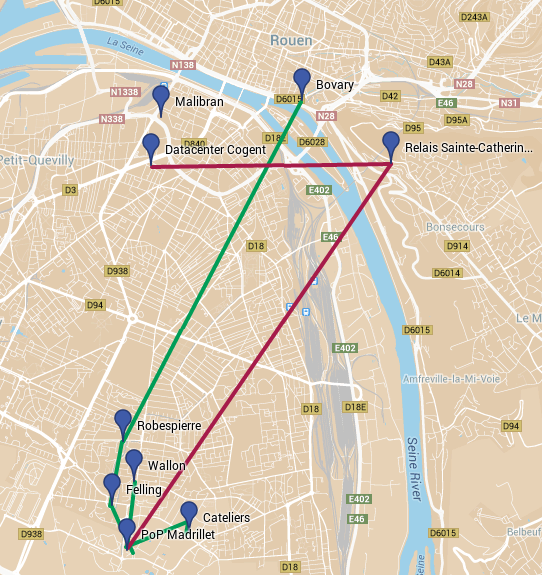
\includegraphics[width=0.70\textwidth]{images/futurReseau.png}
		\end{center}
		
		\end{frame}

	\subsection{Fixation d'une antenne}
		\begin{frame}
		\frametitle{Fixation d'une antenne}
		\vspace{-5px}
		\begin{center}
			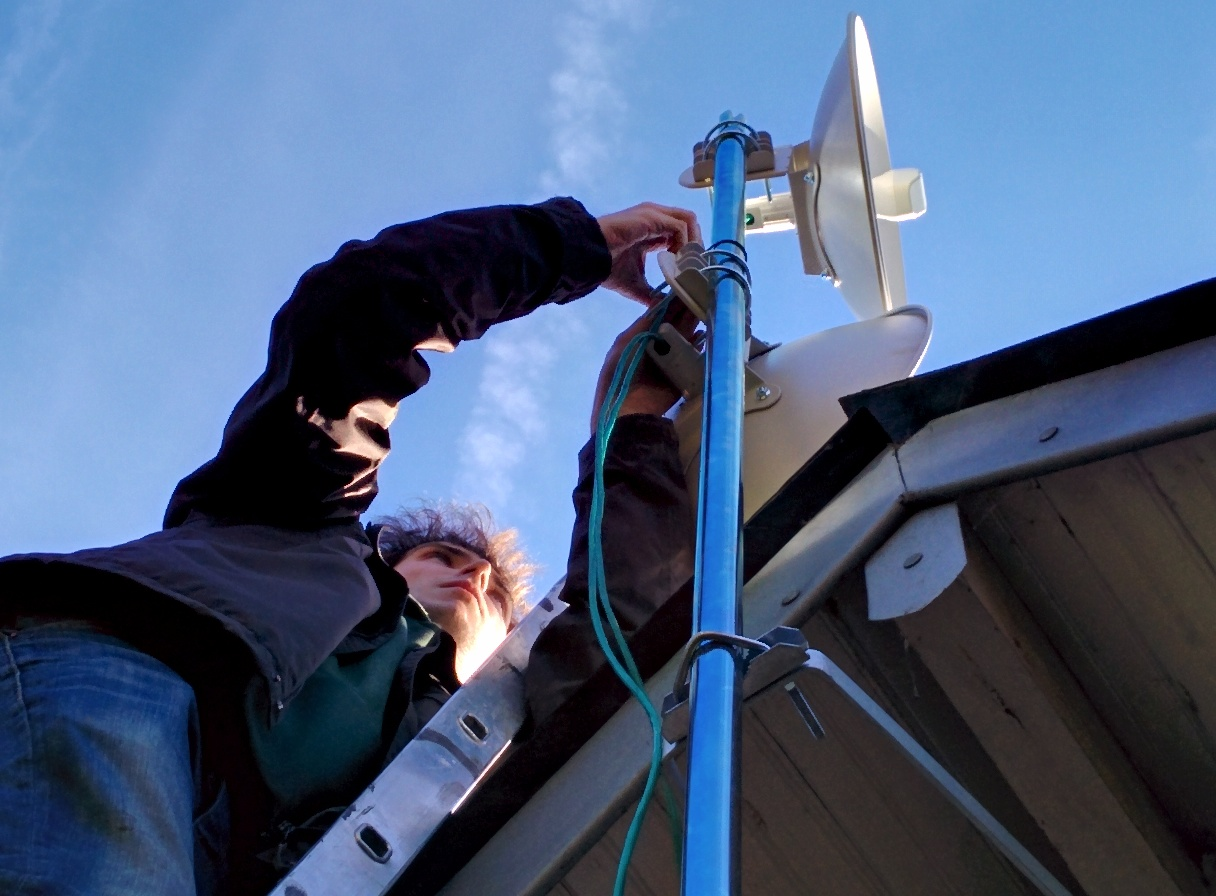
\includegraphics[width=0.75\textwidth]{images/jossAntenne.jpg}
		\end{center}
		
		\end{frame}

	\subsection{Exemple d'antennes}
		\begin{frame}
		\frametitle{Exemple d'antennes}
		\begin{tabular}{l l}
			\begin{minipage}{0.4\textwidth}
				\begin{center}
					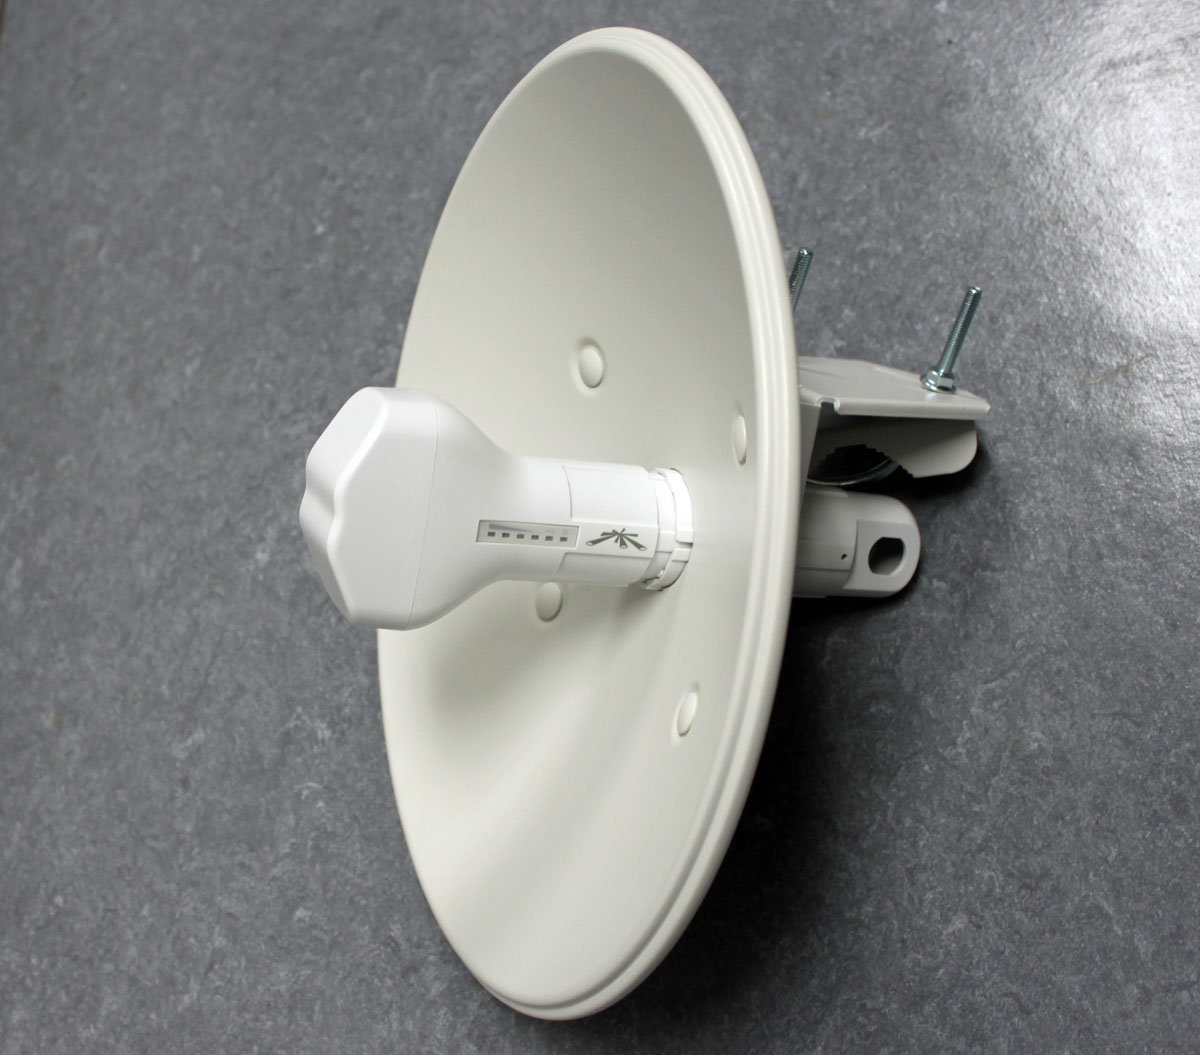
\includegraphics[width=0.95\textwidth]{images/nanobridge.jpg}
				\end{center}
			\end{minipage}

			\begin{minipage}{0.6\textwidth}
				\begin{itemize}
					\item antennes point à point, unidirectionnelles
					\item puissance d'émission inférieure à un téléphone portable (1 W)
					\item longue portée : jusqu'à 15km sans obstacle
					\item prix relativement correct
				\end{itemize}
			\end{minipage}
			
		\end{tabular}
		\end{frame}
	% ///////////////////////////////////////////////////////// %

	% //////////////////////////////////////////// %
	% /// Le sytème d'information /////////////// %
	\section{Le sytème d'information}

	\subsection{Automatiser à l'extrême}
		\begin{frame}
		\frametitle{Automatiser à l'extrême}
		\begin{tabular}{l l}
			\begin{minipage}{0.2\textwidth}
				\begin{center}
					
\includegraphics[width=0.9\textwidth]{images/serveur.png}
				\end{center}
			\end{minipage}

			\begin{minipage}{0.8\textwidth}
				\begin{itemize}
					\item automatiser les adhésions
					\item automatiser l'assistance (hotline, tickets, incidents, brèves)
					\item outils de suivi : assistance et paiements
					\item de l'adhésion à la connexion fonctionnelle dans l'appartement : \mbox{\textbf{2 minutes}}
				\end{itemize}
			\end{minipage}
			
		\end{tabular}
		\end{frame}

	\subsection{L'assistance}
		\begin{frame}
		\frametitle{L'assistance}
		\begin{tabular}{l l}
			\begin{minipage}{0.2\textwidth}
				\begin{center}
					
\includegraphics[width=0.9\textwidth]{images/support.png}
				\end{center}
			\end{minipage}

			\begin{minipage}{0.8\textwidth}
				\begin{itemize}
					\item le plus coûteux en temps et en humain
					\item 90 \% des problèmes ne viennent pas de nous
					\item depuis septembre : 500 tickets / 300 appels
					\begin{itemize}
						\item problèmes d'infrastructure
						\item coupures de courant
						\item pertubations des ondes (Wi-Fi ou AirMax)
						\item prises RJ-45 mal câblées
					\end{itemize}
				\end{itemize}
			\end{minipage}
			
		\end{tabular}
		\end{frame}

	\placelogofalse 
	\subsection{Questions}
		\begin{frame}
		\frametitle{Questions}
		\huge{On vous écoute :)}
		\begin{center}
			
\includegraphics[height=.3\textheight]{images/logo.png}
		\end{center}
		\begin{center}
			\small{\underline{www.quantic-telecom.net}}
		\end{center}
		\end{frame}

	% ///////////////////////////////////////////////////////// %

% Fin du document
\end{document}
